\documentclass[handout]{beamer}
\usetheme[titleprogressbar]{m}

%\usepackage{pgfpages}
%%\setbeameroption{show notes}
%\setbeameroption{show notes on second screen=right}


\setbeamertemplate{caption}[numbered]

\usepackage{graphicx}
\usepackage{multimedia}
%\usepackage[latin1]{inputenc}
\setbeamercovered{transparent}
\usepackage{pgfplots}
\usepackage{pgfplotstable}
\usepackage{color}
\usepackage{subfigure}

\definecolor{OliveGreen}{cmyk}{0.64,0,0.95,0.40}

\usepackage{listings}
\lstset{
    language=Python,
    basicstyle=\tiny\ttfamily,
    commentstyle=\color{OliveGreen}\ttfamily,
    rulecolor=\color{black},
    upquote=true,
    stepnumber=1,
    numbersep=8pt,
    showstringspaces=false,
    breaklines=true,
    frameround=ftff,
    belowcaptionskip=5em,
    belowskip=3em,
    xleftmargin=-2.0cm,
    frame=false,
    framesep=0pt,
    framerule=0pt,
}

\usepackage{tikz}
\usetikzlibrary{calc, matrix, arrows, arrows.meta, automata, shapes, positioning, shadows, trees}

\definecolor{myyellow}{RGB}{240,217,1}
\definecolor{mygreen}{RGB}{143,188,103}
\definecolor{myred}{RGB}{234,38,40}
\definecolor{myblue}{RGB}{53,101,167}

\tikzset{basic/.style={draw}}
\tikzset{input/.style={basic, circle}}
\tikzset{bias/.style={basic, rectangle}}
\tikzset{neuron/.style={basic, circle}}
\tikzset{>=stealth, font=\scriptsize}
\tikzset{sectors/.style n args={2}{%
     circle, draw, minimum width=3.444em,
     append after command={%
         \pgfextra{ %
            \draw (\tikzlastnode.north) -- (\tikzlastnode.south);
            \path (\tikzlastnode.center) -- node[] {#1} (\tikzlastnode.west);
            \path (\tikzlastnode.center) -- node[] {#2} (\tikzlastnode.east);
         }
      }
   }
}

% Beamer stuff
\newcommand\ppbb{path picture bounding box}
\setbeamerfont{bibliography item}{size=\tiny}
\setbeamerfont{bibliography entry author}{size=\tiny}
\setbeamerfont{bibliography entry title}{size=\tiny}
\setbeamerfont{bibliography entry location}{size=\tiny}
\setbeamerfont{bibliography entry note}{size=\tiny}

% argmin
\newcommand{\argmin}[1]{\underset{#1}{\operatorname{arg}\,\operatorname{min}}\;}
% argmax
\newcommand{\argmax}[1]{\underset{#1}{\operatorname{arg}\,\operatorname{max}}\;}

\title[\insertdate]{From Linear Algebra\\to Machine Learning}

\author{Omar Guti\'errez}
\institute{@trinogz}
\date{\today}

\begin{document}

\maketitle

\begin{frame}
    \frametitle{Overview}
    \tableofcontents
\end{frame}


\section{Motivation}
\begin{frame}{Motivation}
    \begin{itemize}
        \item \textbf{Linear algebra} is important to understand machine learning.
        \item As well as \textbf{calculus}, \textbf{probability theory}, and \textbf{statistics}.
        \item It is rewarding to take the \textbf{hard path} to learn machine learning (IMHO).
    \end{itemize}
\end{frame}


%\begin{frame}{Vectorization}
%    \begin{itemize}
%        \item \textbf{ToDo:} Write an introduction to vectorization.
%    \end{itemize}
%\end{frame}


\section{Tensors}
\subsection{Vectors}

\begin{frame}[fragile]{Vectors - \textit{rank-1 tensors}}
    \begin{itemize}
        \item A vector is a collection of numbers
    \end{itemize}
    \begin{columns}
        %%%%%%%%%%%%%%%%%%%%%%%%%%%%%%%%%%%%%%%%%%%%%%%%%%%%%%%%%%%%%%%%%%%%%%
        \begin{column}{0.5\textwidth}
    \large
    \begin{align*} 
        \textcolor{blue}{\vec{a} = \boldsymbol{a}} &= \begin{bmatrix}
           a_{1}  \\
           a_{2}  \\
           \vdots \\
           a_{n}  
         \end{bmatrix}\\
         \begin{bmatrix}
             a_{1}  & a_{2}  & \vdots & a_{n}  
         \end{bmatrix}
    \end{align*}
        \end{column}
        %%%%%%%%%%%%%%%%%%%%%%%%%%%%%%%%%%%%%%%%%%%%%%%%%%%%%%%%%%%%%%%%%%%%%%
        \begin{column}{0.5\textwidth}
            \begin{alertblock}{NumPy}
                \begin{lstlisting}
                # simple vector definition
                a = np.array((5, 4, 3, 2, 1))
                #  shape and size 
                a.shape
                a.size
                # zeros
                np.zeros((5, 5))
                # ones
                np.ones((5, 5))
                # matrix
                np.matrix([[1, 0], [0, 1]])
                \end{lstlisting}
            \end{alertblock}
        \end{column}
        %%%%%%%%%%%%%%%%%%%%%%%%%%%%%%%%%%%%%%%%%%%%%%%%%%%%%%%%%%%%%%%%%%%%%%
        % there are other aspects to take into account, for example, the indexing, appending, reshape, element wise operations
    \end{columns}
\end{frame}

% regularization,
% cost function
% l2 norm in svm

\begin{frame}[fragile]{Norms - $L^p$}
    \begin{columns}
        %%%%%%%%%%%%%%%%%%%%%%%%%%%%%%%%%%%%%%%%%%%%%%%%%%%%%%%%%%%%%%%%%%%%%%
        \begin{column}{0.5\textwidth}
        \huge
            \begin{align*}
                ||\boldsymbol{a}||_p = \Bigg( \sum^{n}_{i=1}̣ |a_i|^p\Bigg)^\frac{1}{p}
            \end{align*}
        \end{column}
        %%%%%%%%%%%%%%%%%%%%%%%%%%%%%%%%%%%%%%%%%%%%%%%%%%%%%%%%%%%%%%%%%%%%%%
        \begin{column}{0.5\textwidth}
            \begin{alertblock}{NumPy}
                \begin{lstlisting}
                np.linalg.norm(a)
                \end{lstlisting}
            \end{alertblock}
            \begin{alertblock}{TensorFlow}
                \begin{lstlisting}
                tf.linalg.norm(a, ord=1)
                tf.norm(a)
                \end{lstlisting}
            \end{alertblock}
        \end{column}
        %%%%%%%%%%%%%%%%%%%%%%%%%%%%%%%%%%%%%%%%%%%%%%%%%%%%%%%%%%%%%%%%%%%%%%
    \end{columns}
\end{frame}


% when we use max norm and L1 norm?
% Frobenius norm for matrices

\begin{frame}[fragile]{Length of a vector - $L^2$ norm}
    \begin{columns}
        %%%%%%%%%%%%%%%%%%%%%%%%%%%%%%%%%%%%%%%%%%%%%%%%%%%%%%%%%%%%%%%%%%%%%%
        \begin{column}{0.5\textwidth}
        \huge
            \begin{align*}
                ||\boldsymbol{a}||_2 &= \Bigg( \sum^{n}_{i=1}̣ |a_i|^2\Bigg)^\frac{1}{2}\\
                                     &= \sqrt{\sum^{n}_{i=1} a_i^2}
            \end{align*}
        \end{column}
        %%%%%%%%%%%%%%%%%%%%%%%%%%%%%%%%%%%%%%%%%%%%%%%%%%%%%%%%%%%%%%%%%%%%%%
        \begin{column}{0.5\textwidth}
            \begin{alertblock}{NumPy}
                \begin{lstlisting}
                np.linalg.norm(a)
                \end{lstlisting}
            \end{alertblock}
            \begin{alertblock}{TensorFlow}
                \begin{lstlisting}
                tf.linalg.norm(a)
                tf.norm(a)
                \end{lstlisting}
            \end{alertblock}
        \end{column}
        %%%%%%%%%%%%%%%%%%%%%%%%%%%%%%%%%%%%%%%%%%%%%%%%%%%%%%%%%%%%%%%%%%%%%%
    \end{columns}
\end{frame}


\begin{frame}[fragile]{Distance between vectors - $L^2$ norm}
    \begin{columns}
        %%%%%%%%%%%%%%%%%%%%%%%%%%%%%%%%%%%%%%%%%%%%%%%%%%%%%%%%%%%%%%%%%%%%%%
        \begin{column}{0.5\textwidth}
    \Large
    \begin{align*}
        d(\boldsymbol{a}, \boldsymbol{b}) &= ||\boldsymbol{a} - \boldsymbol{b}||\\
                                          &= \sqrt{\sum_{i=0}^n (a_{i} - b_{i})^2}
    \end{align*}
        \end{column}
        %%%%%%%%%%%%%%%%%%%%%%%%%%%%%%%%%%%%%%%%%%%%%%%%%%%%%%%%%%%%%%%%%%%%%%
        \begin{column}{0.5\textwidth}
            \begin{alertblock}{NumPy}
                \begin{lstlisting}
                np.linalg.norm(a-b)
                \end{lstlisting}
            \end{alertblock}
            \begin{alertblock}{TensorFlow}
                \begin{lstlisting}
                # Manhattan
                tf.norm(a-b, ord=1)
                # Euclidean
                tf.norm(a-b, ord="euclidean")
                tf.norm(a-b, ord=2)
                \end{lstlisting}
            \end{alertblock}
        \end{column}
        %%%%%%%%%%%%%%%%%%%%%%%%%%%%%%%%%%%%%%%%%%%%%%%%%%%%%%%%%%%%%%%%%%%%%%
    \end{columns}
\end{frame}


% Explain the relationship with norms
% Add visualizations
% Explain that the distances are used for error functions

\begin{frame}[fragile]{More distances}
    \begin{columns}
        %%%%%%%%%%%%%%%%%%%%%%%%%%%%%%%%%%%%%%%%%%%%%%%%%%%%%%%%%%%%%%%%%%%%%%
        \begin{column}{0.5\textwidth}
    \Large
    \begin{align*}
        d(\boldsymbol{a}, \boldsymbol{b}) &= ||\boldsymbol{a} - \boldsymbol{b}||\\
                                          &= \sqrt{\sum_{i=0}^n (a_{i} - b_{i})^2}
    \end{align*}
        \end{column}
        %%%%%%%%%%%%%%%%%%%%%%%%%%%%%%%%%%%%%%%%%%%%%%%%%%%%%%%%%%%%%%%%%%%%%%
        \begin{column}{0.5\textwidth}
            \begin{alertblock}{NumPy}
                \begin{lstlisting}
                np.linalg.norm(a-b)
                \end{lstlisting}
            \end{alertblock}
            \begin{alertblock}{TensorFlow}
                \begin{lstlisting}
                # Manhattan
                tf.norm(a-b, ord=1)
                # Euclidean
                tf.norm(a-b, ord="euclidean")
                tf.norm(a-b, ord=2)
                \end{lstlisting}
            \end{alertblock}
        \end{column}
        %%%%%%%%%%%%%%%%%%%%%%%%%%%%%%%%%%%%%%%%%%%%%%%%%%%%%%%%%%%%%%%%%%%%%%
    \end{columns}
\end{frame}


\begin{frame}[fragile]{Dot product}
    \begin{columns}
        %%%%%%%%%%%%%%%%%%%%%%%%%%%%%%%%%%%%%%%%%%%%%%%%%%%%%%%%%%%%%%%%%%%%%%
        \begin{column}{0.5\textwidth}
            \large
            \begin{align*}
                \textcolor{red}{a \cdot b} &= \textcolor{brown}{\sum_{i=0}^{n} a_i b_i} \\
                                           &= \textcolor{blue}{a_0b_0 + a_1b_1 + \ldots + a_nb_n}
            \end{align*}
        \end{column}
        %%%%%%%%%%%%%%%%%%%%%%%%%%%%%%%%%%%%%%%%%%%%%%%%%%%%%%%%%%%%%%%%%%%%%%
        \begin{column}{0.5\textwidth}
            \begin{alertblock}{NumPy}
                \begin{lstlisting}
                # do not confuse with np.multiply
                np.dot(a, b)
                # or with complex-conjugation
                np.vdot(a, b)
                # or 
                np.sum(np.multiply(a, b))
                \end{lstlisting}
            \end{alertblock}
            \begin{alertblock}{TensorFlow}
                \begin{lstlisting}
                tf.tensordot(a, b, 1)
                # or
                tf.matmul(tf.transpose(a), b)
                # or
                tf.matmul(a, b, transpose_a=True)
                \end{lstlisting}
            \end{alertblock}
        \end{column}
        %%%%%%%%%%%%%%%%%%%%%%%%%%%%%%%%%%%%%%%%%%%%%%%%%%%%%%%%%%%%%%%%%%%%%%
    \end{columns}
\end{frame}


\begin{frame}[fragile]{Dot product and norms}
    \begin{columns}
        %%%%%%%%%%%%%%%%%%%%%%%%%%%%%%%%%%%%%%%%%%%%%%%%%%%%%%%%%%%%%%%%%%%%%%
        \begin{column}{0.5\textwidth}
            So,
            \begin{align*}
                \textcolor{red}{a \cdot a} &= a_0a_0 + a_1a_1 + \ldots + a_na_n \\
                                           &= a_0^2  + a_1^2  + \ldots + a_n^2 \\
                                           &= |\boldsymbol{a}|^2
            \end{align*}
        \end{column}
        %%%%%%%%%%%%%%%%%%%%%%%%%%%%%%%%%%%%%%%%%%%%%%%%%%%%%%%%%%%%%%%%%%%%%%
        \begin{column}{0.5\textwidth}
            \begin{alertblock}{}
                \begin{lstlisting}
                np.linalg.norm(a) ** 2
                # or 
                np.vdot(a, a)
                \end{lstlisting}
            \end{alertblock}
        \end{column}
        %%%%%%%%%%%%%%%%%%%%%%%%%%%%%%%%%%%%%%%%%%%%%%%%%%%%%%%%%%%%%%%%%%%%%%
    \end{columns}
\end{frame}

\begin{frame}[fragile]{Unit vectors}
    \begin{itemize}
        \item \textbf{ToDo}.
        \item Normalization: $\textcolor{blue}{\frac{x}{||x||_2}}$
    \end{itemize}
\end{frame}

\begin{frame}[fragile]{Orthogonality}
    \begin{itemize}
        \item \textbf{ToDo}.
        \item $\textcolor{blue}{\bold{x}^\top\bold{y} = 0}$
        \item When two unit vectors are orthogonal are called \textbf{orthonormal}.
    \end{itemize}
\end{frame}


\subsection{Matrices}
\begin{frame}[fragile]{Matrix - \textit{rank-2 tensors}}
    \begin{itemize}
        \item Matrix multiplication is not commutative. $AB \neq BA$ in general.
    \end{itemize}
    \begin{columns}
        %%%%%%%%%%%%%%%%%%%%%%%%%%%%%%%%%%%%%%%%%%%%%%%%%%%%%%%%%%%%%%%%%%%%%%
        \begin{column}{0.5\textwidth}
            \begin{figure}[htb]
                \centering
                \resizebox{5cm}{6cm}{
                    \input{diagrams/dot_product.tex}
                }
                \label{fig:matmul}
            \end{figure}
        \end{column}
        %%%%%%%%%%%%%%%%%%%%%%%%%%%%%%%%%%%%%%%%%%%%%%%%%%%%%%%%%%%%%%%%%%%%%%
        \begin{column}{0.5\textwidth}
            \begin{alertblock}{NumPy}
                \begin{lstlisting}
                # matmul vs dot
                np.matmul(a, b)
                \end{lstlisting}
            \end{alertblock}
            \begin{alertblock}{TensorFlow}
                \begin{lstlisting}
                tf.matmul(a, b)
                \end{lstlisting}
            \end{alertblock}
        \end{column}
        %%%%%%%%%%%%%%%%%%%%%%%%%%%%%%%%%%%%%%%%%%%%%%%%%%%%%%%%%%%%%%%%%%%%%%
    \end{columns}
\end{frame}


% write more about diagonal matrices, computationally efficient matrix operations
% symmetric matrix, A = A.T
\begin{frame}[fragile]{More special matrices}
    \begin{itemize}
        \item ToDo
        \item Transpose
        \item Diagonal matrices
        \item Identity matrices
        \item Symmetric matrices % distance matrices
        \item Inverse matrix
    \end{itemize}
\end{frame}


\begin{frame}[fragile]{Vector transformations}
    \begin{itemize}
        \item ToDo
        \item Matrices are sometimes used to represent \textbf{vector transformations}.
        % \item Include some example of matrix transpose
    \end{itemize}
\end{frame}


%\begin{frame}[fragile]{\textit{Rank-3 tensors}}
%\end{frame}

\section{Examples}
\begin{frame}[fragile]
    \frametitle{Linear Regression}
    \begin{figure}[htb]
        \centering
        \input{diagrams/regression.tex}
        \label{fig:regression}
	\end{figure}
\end{frame}


\begin{frame}[fragile]
    \frametitle{Linear Regression}
    \Large
    \begin{itemize}
        \item Linear regression is the Swiss Army Knife of Data Science.
    \end{itemize}
    \begin{align*}
        \argmin{a, b} \sum_i (y_i - (ax_i + b))^2 =
        \argmin{\boldsymbol{w}} || \boldsymbol{Xw} - \boldsymbol{y} ||^{2}
    \end{align*}
\end{frame}


% matrix notation
% ToDo: Add arrows
% https://tex.stackexchange.com/questions/361375/how-to-add-arrow-in-equations-and-matrix
\begin{frame}[fragile]
    \frametitle{Linear Regression}
    \Large
    \begin{itemize}
        \item We want to calculate the $w$ coefficients
    \end{itemize}
    \[ 
    \left(
    \begin{array}{c}
        y_1 \\
        y_2 \\
        \ldots \\
        y_n 
    \end{array}
    \right)
    = 
    \left(
    \begin{array}{ccc}
        1 & x_1 \\
        1 & x_2 \\
        1 & \ldots \\
        1 & x_n 
    \end{array}
    \right)
    \bullet
    \left(
    \begin{array}{ccc}
        w_0 \\
        w_1 \\
    \end{array}
    \right)
    \] 
\end{frame}


\begin{frame}[fragile]
    \frametitle{Linear Regression}
    \Large
    \begin{itemize}
        \item In the simplest case we want to calculate the intercept $a$ and the slope $b$.
    \end{itemize}
    \[ 
    \left(
    \begin{array}{c}
        y_1 \\
        y_2 \\
        \ldots \\
        y_n 
    \end{array}
    \right)
    = 
    \left(
    \begin{array}{ccc}
        1 & x_1 \\
        1 & x_2 \\
        1 & \ldots \\
        1 & x_n 
    \end{array}
    \right)
    \bullet
    \left(
    \begin{array}{ccc}
        a \\
        b \\
    \end{array}
    \right)
    \] 
\end{frame}


\begin{frame}[fragile]
    \frametitle{Linear Regression}
    \Large
    \begin{itemize}
        \item The solution to this optimization problem is:
    \end{itemize}
    \begin{align*}
        \boldsymbol{w^{*}} = (\boldsymbol{X}^T\boldsymbol{X})^{-1}\boldsymbol{X}^{T}\boldsymbol{y}\,.
    \end{align*}
\end{frame}


\begin{frame}[fragile]\frametitle{Simple perceptron}
  \begin{figure}[htb]
        \centering
        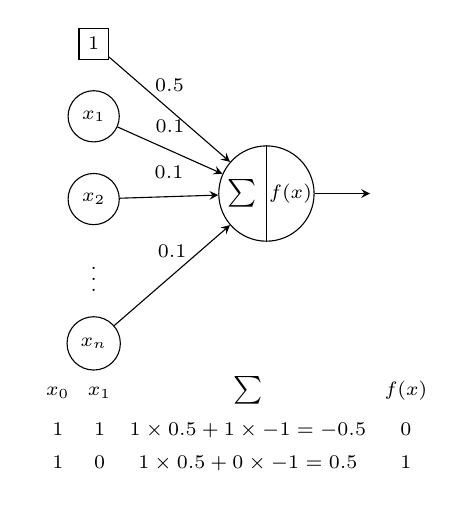
\begin{tikzpicture}[ampersand replacement=\&]

    \node[bias] (bias) {1};
    \node[input, below=1.1em of bias] (i1) {$x_1$};
    \node[input, below=1.1em of i1] (i2) {$x_2$};
    \node[below=0.55em of i2] (idots) {$\vdots$};
    \node[input, below=0.55em of idots] (in) {$x_n$};

    \node[sectors={$\sum$}{$f(x)$}, right=4.5em of bias] (sum) at ($(bias)!0.5!(in)$) {};
    \node[, right=2em of sum] (aux) {};

    \draw[->](bias) to node[above=0.3em] {$0.5$} (sum);
    \draw[->](i1) to node[above=0.3em] {$0.1$} (sum);
    \draw[->](i2) to node[above=0.3em] {$0.1$} (sum);
    \draw[->](in) to node[above=0.3em] {$0.1$} (sum);
    \draw[->](sum) -- (aux);

    \matrix[matrix of nodes, below=7.333em of in] at ($(i1)!0.5!(aux)$) {
        $x_{0}$ \& $x_{1}$ \& $\sum$                              \& $f(x)$ \\
        1       \& 1       \& $1 \times 0.5 + 1 \times -1 = -0.5$ \& 0      \\
        1       \& 0       \& $1 \times 0.5 + 0 \times -1 = 0.5$  \& 1      \\
    };

\end{tikzpicture}

        \label{fig:perceptron}
	\end{figure}
\end{frame}

\begin{frame}[fragile]\frametitle{Neural Networks}
    \begin{itemize}
        \item \textbf{ToDo}.
    \end{itemize}
\end{frame}

\begin{frame}[fragile]\frametitle{Eigendecomposition}
    \Large
    \begin{itemize}
        \item This \textbf{matrix decomposition} technique is the base of \textbf{dimensionality reduction}.
    \end{itemize}
    \begin{align*}
        \boldsymbol{Av} = \lambda \boldsymbol{v}
    \end{align*}
    \begin{itemize}
        \item $\boldsymbol{A}$ (with dimension $N\times N$) is a square matrix
        \item $\boldsymbol{v}$ (with dimension $N$) is the eigenvector
        \item $\lambda$ is a scalar value
    \end{itemize}
\end{frame}

\begin{frame}[fragile]\frametitle{Neural Networks}
    \begin{itemize}
        \item \textbf{ToDo}.
    \end{itemize}
\end{frame}

\section{Conclusions}

\begin{frame}{More topics we should check}
    \begin{itemize}
        \item \textbf{Gradient descent} is a beautiful optimization algorithm,
                basically, we multiply matrices to many times.
        \item Be aware that \textbf{numerical instabilities} can happen, and avoid these ones.
    \end{itemize} 
\end{frame}

\begin{frame}{References}
    \begin{itemize}
        \item \textbf{Mathematics for Machine Learning: Linear Algebra} by Coursera.
        \item \textbf{The Math of Intelligence} by Siraj Raval.
        \item \textbf{Deep Learning Book} by Bengio and Goodfellow, has a chapter summarizing
            which linear algebra topics you need to learn neural networks.
    \end{itemize}
\end{frame}

\begin{frame}
\huge{Thank you.}\\
\huge{Questions?}\\
\huge{Comments?}\\
\end{frame}

\end{document}
